\section{ueac.h File Reference}
\label{ueac_8h}\index{ueac.h@{ueac.h}}


This graph shows which files directly or indirectly include this file:\begin{figure}[H]
\begin{center}
\leavevmode
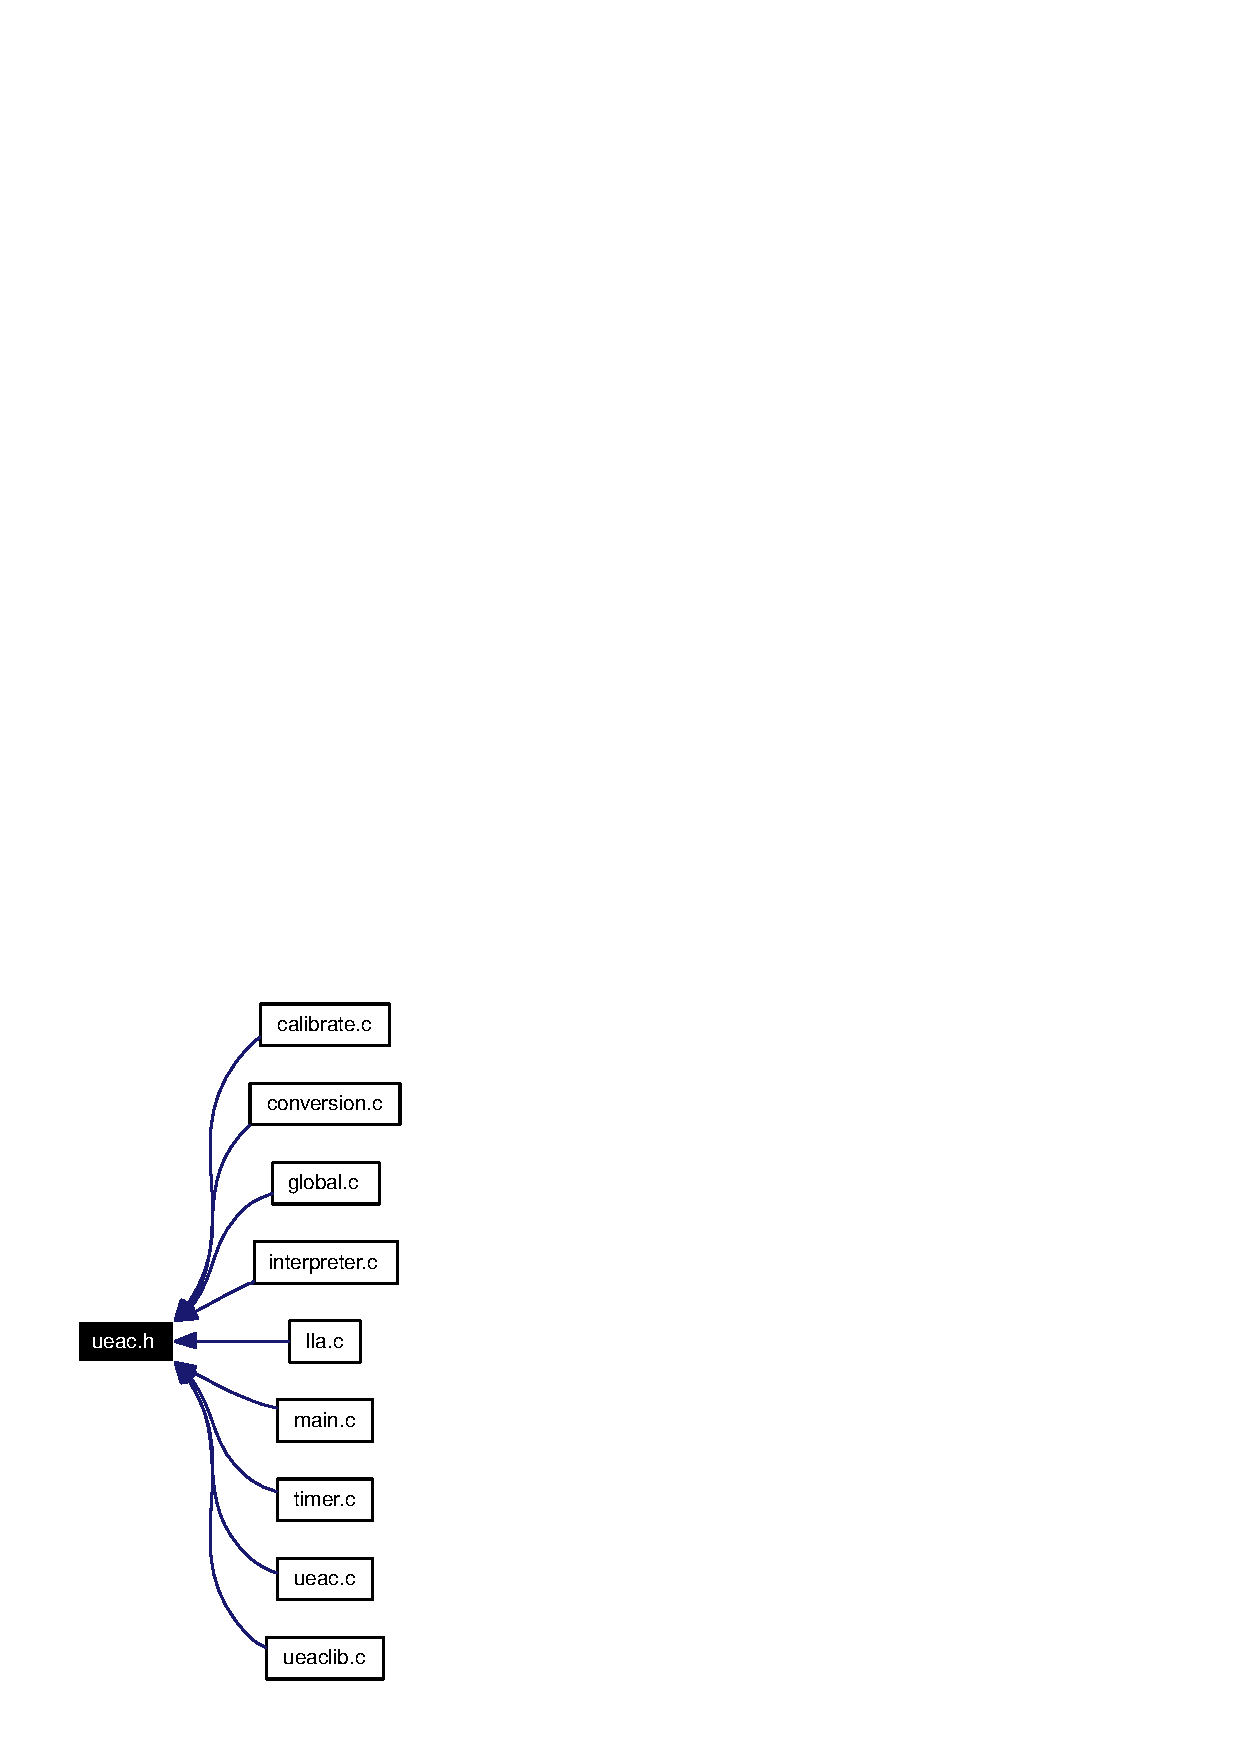
\includegraphics[width=96pt]{ueac_8h__dep__incl}
\end{center}
\end{figure}
\subsection*{Data Structures}
\begin{CompactItemize}
\item 
struct {\bf ueac\_\-instruction}
\item 
struct {\bf lla}
\item 
struct {\bf cal}
\item 
struct {\bf ueac}
\end{CompactItemize}
\subsection*{Defines}
\begin{CompactItemize}
\item 
\#define {\bf VOLTAGE\_\-SENSE}~0x1000
\item 
\#define {\bf I\_\-CONSTANT}~0x2000
\item 
\#define {\bf LLA\_\-IN}~0x4000
\item 
\#define {\bf LLA\_\-OUT}~0x8000
\item 
\#define {\bf UEAC\_\-HALT}~0x01
\item 
\#define {\bf UEAC\_\-RUN}~0x02
\item 
\#define {\bf UEAC\_\-READY}~0x00
\item 
\#define {\bf UEAC\_\-EXECUTE}~0x01
\item 
\#define {\bf UEAC\_\-ALL\_\-V}~0
\item 
\#define {\bf UEAC\_\-ALL\_\-I}~1
\item 
\#define {\bf UEAC\_\-READ\_\-V}~2
\item 
\#define {\bf UEAC\_\-READ\_\-I}~3
\item 
\#define {\bf UEAC\_\-WRITE}~4
\item 
\#define {\bf UEAC\_\-LLA\_\-ADD}~5
\item 
\#define {\bf UEAC\_\-LLA\_\-DISABLE}~6
\item 
\#define {\bf UEAC\_\-LLA\_\-ENABLE}~7
\item 
\#define {\bf UEAC\_\-LLA\_\-REPORT}~8
\item 
\#define {\bf UEAC\_\-RST}~9
\item 
\#define {\bf UEAC\_\-CAL}~10
\item 
\#define {\bf UEAC\_\-LON}~11
\item 
\#define {\bf UEAC\_\-LOF}~12
\end{CompactItemize}
\subsection*{Typedefs}
\begin{CompactItemize}
\item 
typedef {\bf ueac\_\-instruction} {\bf ueac\_\-instruction\_\-t}
\item 
typedef {\bf lla} {\bf lla\_\-t}
\item 
typedef {\bf cal} {\bf cal\_\-t}
\item 
typedef {\bf ueac} {\bf ueac\_\-t}
\end{CompactItemize}
\subsection*{Functions}
\begin{CompactItemize}
\item 
int {\bf init\_\-ueac} ({\bf ueac\_\-t} $\ast$)
\item 
int {\bf display\_\-ueac} ({\bf ueac\_\-t} $\ast$)
\item 
int {\bf ueac\_\-execute\_\-instruction} ({\bf ueac\_\-t} $\ast$)
\item 
int {\bf lla\_\-input\_\-check} (char, {\bf ueac\_\-t} $\ast$)
\end{CompactItemize}


\subsection{Define Documentation}
\index{ueac.h@{ueac.h}!I_CONSTANT@{I\_\-CONSTANT}}
\index{I_CONSTANT@{I\_\-CONSTANT}!ueac.h@{ueac.h}}
\subsubsection{\setlength{\rightskip}{0pt plus 5cm}\#define I\_\-CONSTANT~0x2000}\label{ueac_8h_a1}




Definition at line 48 of file ueac.h.\index{ueac.h@{ueac.h}!LLA_IN@{LLA\_\-IN}}
\index{LLA_IN@{LLA\_\-IN}!ueac.h@{ueac.h}}
\subsubsection{\setlength{\rightskip}{0pt plus 5cm}\#define LLA\_\-IN~0x4000}\label{ueac_8h_a2}




Definition at line 49 of file ueac.h.\index{ueac.h@{ueac.h}!LLA_OUT@{LLA\_\-OUT}}
\index{LLA_OUT@{LLA\_\-OUT}!ueac.h@{ueac.h}}
\subsubsection{\setlength{\rightskip}{0pt plus 5cm}\#define LLA\_\-OUT~0x8000}\label{ueac_8h_a3}




Definition at line 50 of file ueac.h.\index{ueac.h@{ueac.h}!UEAC_ALL_I@{UEAC\_\-ALL\_\-I}}
\index{UEAC_ALL_I@{UEAC\_\-ALL\_\-I}!ueac.h@{ueac.h}}
\subsubsection{\setlength{\rightskip}{0pt plus 5cm}\#define UEAC\_\-ALL\_\-I~1}\label{ueac_8h_a9}




Definition at line 62 of file ueac.h.

Referenced by interpreter(), and ueac\_\-execute\_\-instruction().\index{ueac.h@{ueac.h}!UEAC_ALL_V@{UEAC\_\-ALL\_\-V}}
\index{UEAC_ALL_V@{UEAC\_\-ALL\_\-V}!ueac.h@{ueac.h}}
\subsubsection{\setlength{\rightskip}{0pt plus 5cm}\#define UEAC\_\-ALL\_\-V~0}\label{ueac_8h_a8}




Definition at line 61 of file ueac.h.

Referenced by interpreter(), and ueac\_\-execute\_\-instruction().\index{ueac.h@{ueac.h}!UEAC_CAL@{UEAC\_\-CAL}}
\index{UEAC_CAL@{UEAC\_\-CAL}!ueac.h@{ueac.h}}
\subsubsection{\setlength{\rightskip}{0pt plus 5cm}\#define UEAC\_\-CAL~10}\label{ueac_8h_a18}




Definition at line 71 of file ueac.h.

Referenced by interpreter(), and ueac\_\-execute\_\-instruction().\index{ueac.h@{ueac.h}!UEAC_EXECUTE@{UEAC\_\-EXECUTE}}
\index{UEAC_EXECUTE@{UEAC\_\-EXECUTE}!ueac.h@{ueac.h}}
\subsubsection{\setlength{\rightskip}{0pt plus 5cm}\#define UEAC\_\-EXECUTE~0x01}\label{ueac_8h_a7}




Definition at line 58 of file ueac.h.

Referenced by interpreter(), and ueac\_\-execute\_\-instruction().\index{ueac.h@{ueac.h}!UEAC_HALT@{UEAC\_\-HALT}}
\index{UEAC_HALT@{UEAC\_\-HALT}!ueac.h@{ueac.h}}
\subsubsection{\setlength{\rightskip}{0pt plus 5cm}\#define UEAC\_\-HALT~0x01}\label{ueac_8h_a4}




Definition at line 53 of file ueac.h.\index{ueac.h@{ueac.h}!UEAC_LLA_ADD@{UEAC\_\-LLA\_\-ADD}}
\index{UEAC_LLA_ADD@{UEAC\_\-LLA\_\-ADD}!ueac.h@{ueac.h}}
\subsubsection{\setlength{\rightskip}{0pt plus 5cm}\#define UEAC\_\-LLA\_\-ADD~5}\label{ueac_8h_a13}




Definition at line 66 of file ueac.h.

Referenced by interpreter(), and ueac\_\-execute\_\-instruction().\index{ueac.h@{ueac.h}!UEAC_LLA_DISABLE@{UEAC\_\-LLA\_\-DISABLE}}
\index{UEAC_LLA_DISABLE@{UEAC\_\-LLA\_\-DISABLE}!ueac.h@{ueac.h}}
\subsubsection{\setlength{\rightskip}{0pt plus 5cm}\#define UEAC\_\-LLA\_\-DISABLE~6}\label{ueac_8h_a14}




Definition at line 67 of file ueac.h.

Referenced by interpreter(), and ueac\_\-execute\_\-instruction().\index{ueac.h@{ueac.h}!UEAC_LLA_ENABLE@{UEAC\_\-LLA\_\-ENABLE}}
\index{UEAC_LLA_ENABLE@{UEAC\_\-LLA\_\-ENABLE}!ueac.h@{ueac.h}}
\subsubsection{\setlength{\rightskip}{0pt plus 5cm}\#define UEAC\_\-LLA\_\-ENABLE~7}\label{ueac_8h_a15}




Definition at line 68 of file ueac.h.

Referenced by interpreter(), and ueac\_\-execute\_\-instruction().\index{ueac.h@{ueac.h}!UEAC_LLA_REPORT@{UEAC\_\-LLA\_\-REPORT}}
\index{UEAC_LLA_REPORT@{UEAC\_\-LLA\_\-REPORT}!ueac.h@{ueac.h}}
\subsubsection{\setlength{\rightskip}{0pt plus 5cm}\#define UEAC\_\-LLA\_\-REPORT~8}\label{ueac_8h_a16}




Definition at line 69 of file ueac.h.

Referenced by interpreter(), and ueac\_\-execute\_\-instruction().\index{ueac.h@{ueac.h}!UEAC_LOF@{UEAC\_\-LOF}}
\index{UEAC_LOF@{UEAC\_\-LOF}!ueac.h@{ueac.h}}
\subsubsection{\setlength{\rightskip}{0pt plus 5cm}\#define UEAC\_\-LOF~12}\label{ueac_8h_a20}




Definition at line 73 of file ueac.h.

Referenced by interpreter(), and ueac\_\-execute\_\-instruction().\index{ueac.h@{ueac.h}!UEAC_LON@{UEAC\_\-LON}}
\index{UEAC_LON@{UEAC\_\-LON}!ueac.h@{ueac.h}}
\subsubsection{\setlength{\rightskip}{0pt plus 5cm}\#define UEAC\_\-LON~11}\label{ueac_8h_a19}




Definition at line 72 of file ueac.h.

Referenced by interpreter(), and ueac\_\-execute\_\-instruction().\index{ueac.h@{ueac.h}!UEAC_READ_I@{UEAC\_\-READ\_\-I}}
\index{UEAC_READ_I@{UEAC\_\-READ\_\-I}!ueac.h@{ueac.h}}
\subsubsection{\setlength{\rightskip}{0pt plus 5cm}\#define UEAC\_\-READ\_\-I~3}\label{ueac_8h_a11}




Definition at line 64 of file ueac.h.

Referenced by interpreter(), and ueac\_\-execute\_\-instruction().\index{ueac.h@{ueac.h}!UEAC_READ_V@{UEAC\_\-READ\_\-V}}
\index{UEAC_READ_V@{UEAC\_\-READ\_\-V}!ueac.h@{ueac.h}}
\subsubsection{\setlength{\rightskip}{0pt plus 5cm}\#define UEAC\_\-READ\_\-V~2}\label{ueac_8h_a10}




Definition at line 63 of file ueac.h.

Referenced by interpreter(), and ueac\_\-execute\_\-instruction().\index{ueac.h@{ueac.h}!UEAC_READY@{UEAC\_\-READY}}
\index{UEAC_READY@{UEAC\_\-READY}!ueac.h@{ueac.h}}
\subsubsection{\setlength{\rightskip}{0pt plus 5cm}\#define UEAC\_\-READY~0x00}\label{ueac_8h_a6}




Definition at line 57 of file ueac.h.

Referenced by ueac\_\-execute\_\-instruction().\index{ueac.h@{ueac.h}!UEAC_RST@{UEAC\_\-RST}}
\index{UEAC_RST@{UEAC\_\-RST}!ueac.h@{ueac.h}}
\subsubsection{\setlength{\rightskip}{0pt plus 5cm}\#define UEAC\_\-RST~9}\label{ueac_8h_a17}




Definition at line 70 of file ueac.h.

Referenced by interpreter(), and ueac\_\-execute\_\-instruction().\index{ueac.h@{ueac.h}!UEAC_RUN@{UEAC\_\-RUN}}
\index{UEAC_RUN@{UEAC\_\-RUN}!ueac.h@{ueac.h}}
\subsubsection{\setlength{\rightskip}{0pt plus 5cm}\#define UEAC\_\-RUN~0x02}\label{ueac_8h_a5}




Definition at line 54 of file ueac.h.\index{ueac.h@{ueac.h}!UEAC_WRITE@{UEAC\_\-WRITE}}
\index{UEAC_WRITE@{UEAC\_\-WRITE}!ueac.h@{ueac.h}}
\subsubsection{\setlength{\rightskip}{0pt plus 5cm}\#define UEAC\_\-WRITE~4}\label{ueac_8h_a12}




Definition at line 65 of file ueac.h.

Referenced by interpreter(), and ueac\_\-execute\_\-instruction().\index{ueac.h@{ueac.h}!VOLTAGE_SENSE@{VOLTAGE\_\-SENSE}}
\index{VOLTAGE_SENSE@{VOLTAGE\_\-SENSE}!ueac.h@{ueac.h}}
\subsubsection{\setlength{\rightskip}{0pt plus 5cm}\#define VOLTAGE\_\-SENSE~0x1000}\label{ueac_8h_a0}




Definition at line 47 of file ueac.h.

\subsection{Typedef Documentation}
\index{ueac.h@{ueac.h}!cal_t@{cal\_\-t}}
\index{cal_t@{cal\_\-t}!ueac.h@{ueac.h}}
\subsubsection{\setlength{\rightskip}{0pt plus 5cm}typedef struct {\bf cal}  {\bf cal\_\-t}}\label{ueac_8h_a23}


\index{ueac.h@{ueac.h}!lla_t@{lla\_\-t}}
\index{lla_t@{lla\_\-t}!ueac.h@{ueac.h}}
\subsubsection{\setlength{\rightskip}{0pt plus 5cm}typedef struct {\bf lla}  {\bf lla\_\-t}}\label{ueac_8h_a22}


\index{ueac.h@{ueac.h}!ueac_instruction_t@{ueac\_\-instruction\_\-t}}
\index{ueac_instruction_t@{ueac\_\-instruction\_\-t}!ueac.h@{ueac.h}}
\subsubsection{\setlength{\rightskip}{0pt plus 5cm}typedef struct {\bf ueac\_\-instruction}  {\bf ueac\_\-instruction\_\-t}}\label{ueac_8h_a21}


\index{ueac.h@{ueac.h}!ueac_t@{ueac\_\-t}}
\index{ueac_t@{ueac\_\-t}!ueac.h@{ueac.h}}
\subsubsection{\setlength{\rightskip}{0pt plus 5cm}typedef struct {\bf ueac}  {\bf ueac\_\-t}}\label{ueac_8h_a24}




\subsection{Function Documentation}
\index{ueac.h@{ueac.h}!display_ueac@{display\_\-ueac}}
\index{display_ueac@{display\_\-ueac}!ueac.h@{ueac.h}}
\subsubsection{\setlength{\rightskip}{0pt plus 5cm}int display\_\-ueac ({\bf ueac\_\-t} $\ast$)}\label{ueac_8h_a26}


\index{ueac.h@{ueac.h}!init_ueac@{init\_\-ueac}}
\index{init_ueac@{init\_\-ueac}!ueac.h@{ueac.h}}
\subsubsection{\setlength{\rightskip}{0pt plus 5cm}int init\_\-ueac ({\bf ueac\_\-t} $\ast$)}\label{ueac_8h_a25}


\index{ueac.h@{ueac.h}!lla_input_check@{lla\_\-input\_\-check}}
\index{lla_input_check@{lla\_\-input\_\-check}!ueac.h@{ueac.h}}
\subsubsection{\setlength{\rightskip}{0pt plus 5cm}int lla\_\-input\_\-check (char, {\bf ueac\_\-t} $\ast$)}\label{ueac_8h_a28}


\index{ueac.h@{ueac.h}!ueac_execute_instruction@{ueac\_\-execute\_\-instruction}}
\index{ueac_execute_instruction@{ueac\_\-execute\_\-instruction}!ueac.h@{ueac.h}}
\subsubsection{\setlength{\rightskip}{0pt plus 5cm}int ueac\_\-execute\_\-instruction ({\bf ueac\_\-t} $\ast$)}\label{ueac_8h_a27}




Definition at line 64 of file ueac.c.

References clear\_\-led\_\-screen(), ueac\_\-instruction::command\_\-reg, conversion\_\-result, convert\_\-a2d(), current\_\-output\_\-calibration(), ueacval::hundredth, I\_\-CONVERSION, lla\_\-data::input, ueac::instruction, ueac\_\-instruction::instruction\_\-type, ueacval::integer, led\_\-screen\_\-enable, lla\_\-add(), lla\_\-disable(), lla\_\-enable(), lla\_\-input\_\-check(), lla\_\-report(), lla\_\-data::output, ueac::pin\_\-current, pin\_\-data, ueac\_\-instruction::pin\_\-x, ueac\_\-instruction::pin\_\-y, system\_\-reset(), UEAC\_\-ALL\_\-I, UEAC\_\-ALL\_\-V, UEAC\_\-CAL, UEAC\_\-EXECUTE, UEAC\_\-LLA\_\-ADD, UEAC\_\-LLA\_\-DISABLE, UEAC\_\-LLA\_\-ENABLE, UEAC\_\-LLA\_\-REPORT, UEAC\_\-LOF, UEAC\_\-LON, UEAC\_\-READ\_\-I, UEAC\_\-READ\_\-V, UEAC\_\-READY, UEAC\_\-RST, ueac\_\-state, UEAC\_\-WRITE, V\_\-CONVERSION, ueac\_\-instruction::value, and write\_\-current().

Referenced by interpreter().

\footnotesize\begin{verbatim}64                                                    {
65   enum {OFF,ON};
66   int return_val=0;
67 
68 #ifndef LINUX
69   int i;
70   int probe_num;
71 #endif 
72   if (system_state->instruction.command_reg==UEAC_EXECUTE) {
73     switch (system_state->instruction.instruction_type) {
74     case UEAC_ALL_V:
75 #ifndef LINUX
76       for (i=0;i<25;i++) {
77         if (lla_input_check(i,system_state)) {
78           convert_a2d(I_CONVERSION,pin_data[i].filtered_result,&conversion_result,i);
79           printf("0.%03d,",conversion_result.integer);
80         }
81         else {
82           convert_a2d(V_CONVERSION,pin_data[i].filtered_result,&conversion_result,i);
83           printf("%d.%02d,",conversion_result.integer,conversion_result.hundredth);
84         }
85       }
86 #else 
87       printf("UEAC_ALL_V ");
88 #endif
89       break;
90     case UEAC_ALL_I:
91 #ifndef LINUX
92       for (i=0;i<25;i++) {
93         if (lla_input_check(i,system_state)) {
94           convert_a2d(I_CONVERSION,pin_data[i].filtered_result,&conversion_result,i);
95           printf("-%d,",conversion_result.integer);
96         }
97         else {
98           printf("%d,",system_state->pin_current[i]);
99         }
100       }
101 #else 
102       printf("UEAC_ALL_I ");
103 #endif
104       break;
105     case UEAC_READ_V:
106 #ifndef LINUX
107       probe_num=((system_state->instruction.pin_y-1)*5)+(system_state->instruction.pin_x-1);
108       if (lla_input_check(probe_num,system_state)) {
109         convert_a2d(I_CONVERSION,pin_data[probe_num].filtered_result,&conversion_result,probe_num);
110         printf("0.%03d,",conversion_result.integer);
111       }
112       else {
113         convert_a2d(V_CONVERSION,pin_data[probe_num].filtered_result,&conversion_result,probe_num);
114         printf("%d.%02d,",conversion_result.integer,conversion_result.hundredth);
115       }
116 #else 
117       printf("UEAC_READ_V ");
118 #endif
119       break;
120     case UEAC_READ_I:
121 #ifndef LINUX
122       probe_num=((system_state->instruction.pin_y-1)*5)+(system_state->instruction.pin_x-1);
123       if (lla_input_check(probe_num,system_state)) {
124         convert_a2d(I_CONVERSION,pin_data[probe_num].filtered_result,&conversion_result,probe_num);
125         printf("-%d,",conversion_result.integer);
126       }
127       else {
128         printf("%d,",system_state->pin_current[probe_num]);
129       }
130 #else 
131       printf("UEAC_READ_I ");
132 #endif
133       break;
134     case UEAC_WRITE:
135 #ifndef LINUX
136       probe_num=((system_state->instruction.pin_y-1)*5)+(system_state->instruction.pin_x-1);
137       write_current(probe_num,system_state->instruction.value); 
138       system_state->pin_current[probe_num]=system_state->instruction.value;
139 #else 
140       printf("UEAC_WRITE ");
141 #endif
142       break;
143     case UEAC_LLA_ADD:
144       lla_add(system_state);
145 #ifndef LINUX
146 #else 
147       printf("UEAC_LLA_ADD ");
148 #endif
149       break;
150     case UEAC_LLA_DISABLE:
151       lla_disable(system_state);
152 #ifndef LINUX
153 #else 
154       printf("UEAC_LLA_DISABLE ");
155 #endif
156       break;
157     case UEAC_LLA_ENABLE:
158       lla_enable(system_state);
159 #ifndef LINUX
160 #else 
161       printf("UEAC_LLA_ENABLE ");
162 #endif
163       break;
164     case UEAC_LLA_REPORT:
165       if (lla_report(system_state,&lla_data)==0) {
166         printf("-%d,%d,",lla_data.input,lla_data.output);
167       }
168       else {
169         printf("*,*,");
170       }
171 #ifndef LINUX
172 #else 
173       printf("UEAC_LLA_REPORT ");
174 #endif
175       break;
176     case UEAC_CAL:
177 #ifndef LINUX
178       current_output_calibration(&ueac_state);
179 #else 
180       printf("UEAC_CAL ");
181 #endif
182       break;
183     case UEAC_RST:
184 #ifndef LINUX
185       printf("OK\n\r");
186       system_reset();
187 #else 
188       printf("UEAC_RST ");
189 #endif
190       break;
191     case UEAC_LON:
192 #ifndef LINUX
193       led_screen_enable=1;
194 #else 
195       printf("UEAC_LON ");
196 #endif
197       break;
198     case UEAC_LOF:
199 #ifndef LINUX
200       led_screen_enable=0;
201       clear_led_screen();
202 #else 
203       printf("UEAC_LOF ");
204 #endif
205       break;
206     }
207 #ifndef LINUX
208     printf("OK\n\r");
209 #else 
210     printf("OK\n");
211 #endif
212   }
213   else {
214 #ifndef LINUX
215     printf("NOK\n\r");
216 #else 
217     printf("NOK\n");
218 #endif 
219     return_val=1;
220   }
221   system_state->instruction.command_reg=UEAC_READY;
222   return(return_val);
223 }
\end{verbatim}\normalsize 




Here is the call graph for this function:\begin{figure}[H]
\begin{center}
\leavevmode
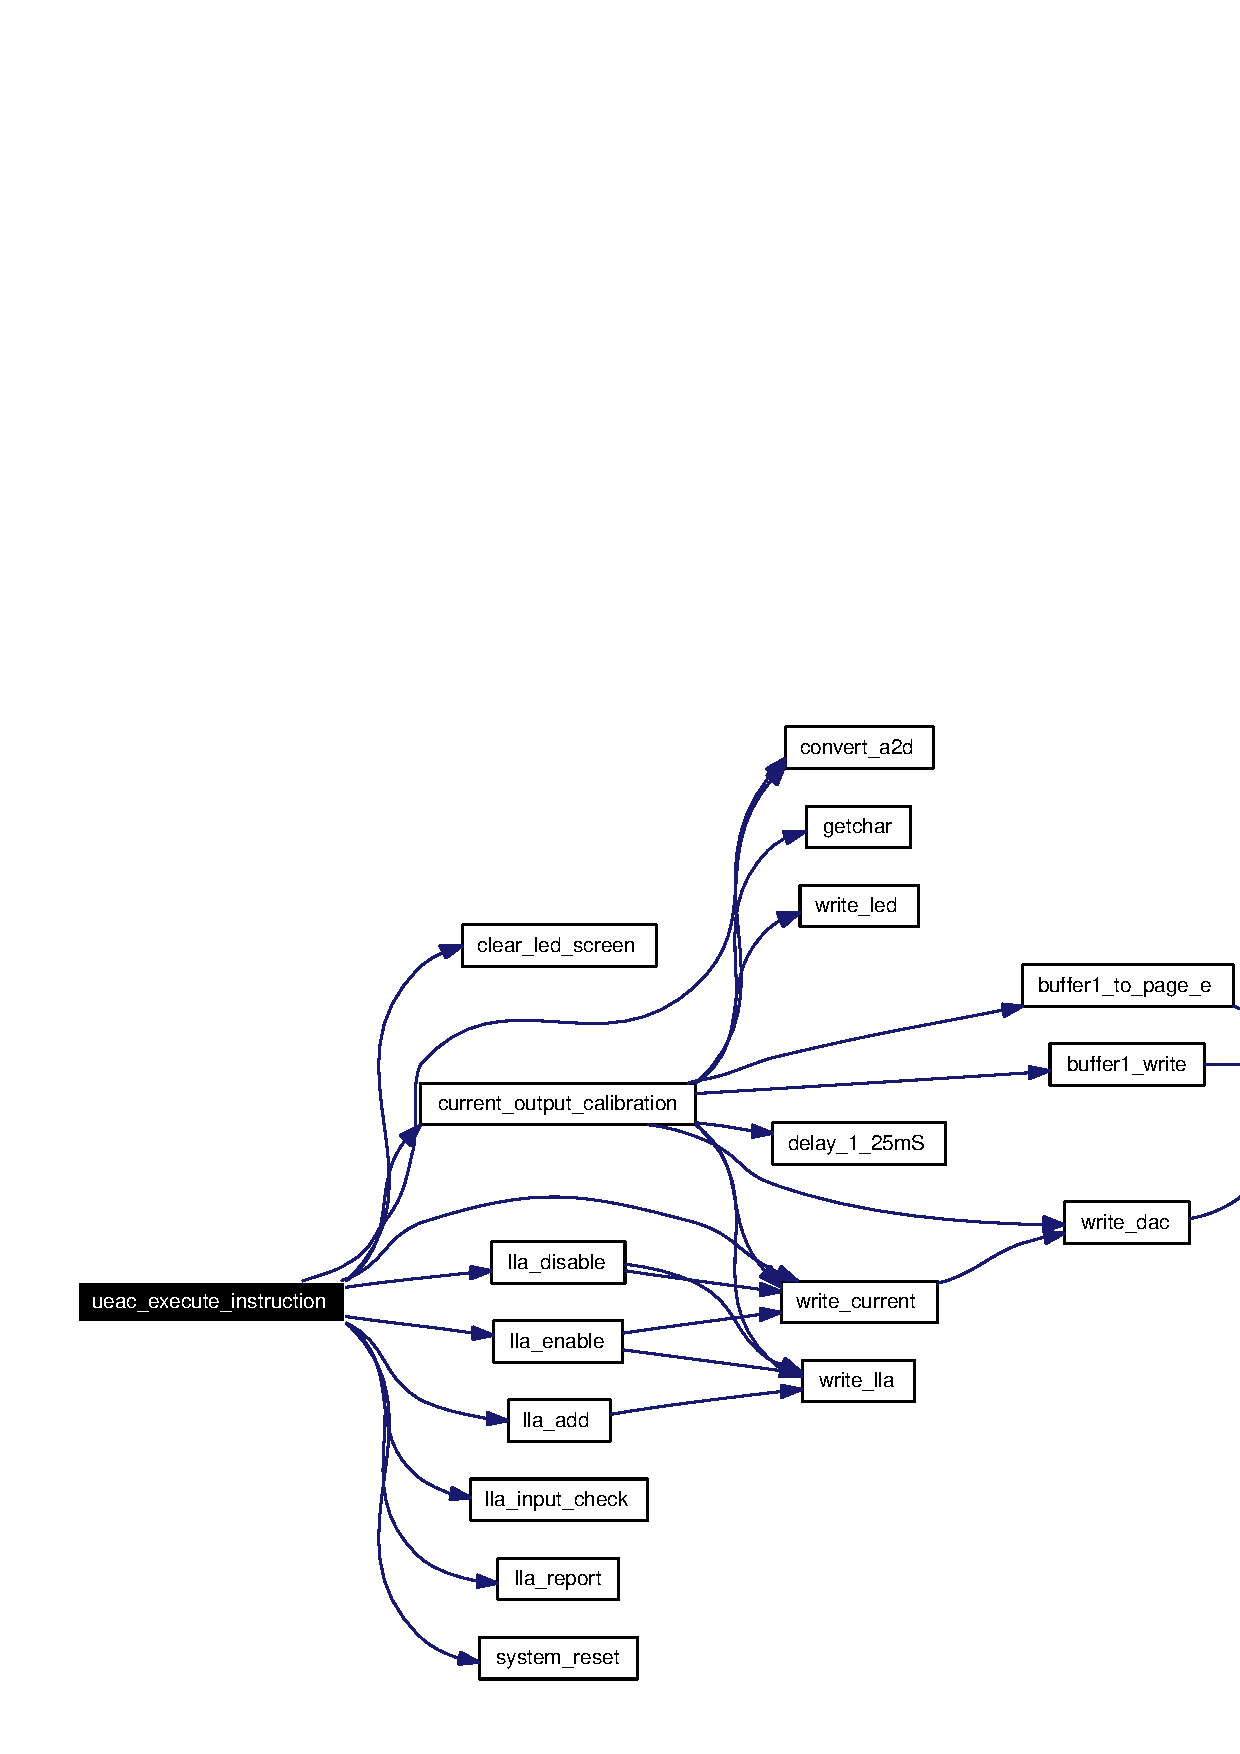
\includegraphics[width=355pt]{ueac_8h_a27_cgraph}
\end{center}
\end{figure}
